% Homework URL: https://zhuoqing.blog.csdn.net/article/details/146195929

\section{Homework 4}

\subsection{卷积运算}

\subsubsection{根据公式或者性质求解卷积}

(1) 
\begin{align*}
    f_1*f_2=\delta(2t)*e^{-t}u(t)+\delta'(t-2)*e^{-t}u(t)=\dfrac{1}{2}e^{-t}u(t)+e^{2-t}[\delta(t)-u(t)]
\end{align*}

(2) 
\begin{align*}
    f_1*f_2=&u(t+1)*u(t+1)-2u(t+1)*u(t-1)+u(t-1)*u(t-1)  \\
    &=f(t+2)-2f(t)+f(t-2)
\end{align*}

其中$f(t)$为单位斜变信号.

(3)
\begin{align*}
    f_1*f_2=&\displaystyle\int_{-\infty}^{t}\cos(\omega t + \frac{\pi}{3})u(t)\mathrm{d}t \\
    =&\left\{
        \begin{array}{ll}
            0 & t < 0 \\
            \dfrac{1}{\omega}\sin(\omega t+\dfrac{\pi}{3})-\dfrac{\sqrt{3}}{2} & \text{otherwise}
        \end{array}
    \right.
\end{align*}

(4) 
\begin{align*}
    f_1*f_2=&\displaystyle\sum_{\tau=n-3}^{n}\sin(\omega_1\tau)u[\tau+2] \\
    =&\left\{\begin{array}{ll}
        0 & n < -2 \\
        \sin(-2\omega_1) & n = -2 \\
        \sin(-2\omega_1)+\sin(-\omega_1) & n = -1 \lor n = 0 \\
        \sin((n-3)\omega_1)+\sin((n-2)\omega_1)+\sin((n-1)\omega_1)+\sin(n\omega_1) & \text{otherwise}
    \end{array}\right.
\end{align*}
\subsubsection{应用图解方法求卷积}

\task{必做题}

\begin{figure*}[htbp]
    \centering
    \includegraphics[width=0.7\textwidth]{images/1-2-essential.png}
    \caption{必做-图解卷积}\label{fig:4-1-2(1)}
\end{figure*}

图解分析如图\ref{fig:4-1-2(1)}所示. 卷积信号的表达式为
\begin{align*}
    f_1*f_2=\left\{
        \begin{array}{ll}
            \dfrac{1}{2}e^{-2(t+1)}-\dfrac{1}{2}e & -1.5 < t < -0.5 \\
            \dfrac{1}{2}e^{-2(t+1)}-\dfrac{1}{2}e^{-2t} & -0.5 < t < 1 \\
            \dfrac{1}{2}e^{-4}-\dfrac{1}{2}e^{-2t} & 1 < t < 2 \\
            0 & \text{otherwise}
        \end{array}
    \right.
\end{align*}

\task{选做题}

图解如图\ref{fig:4-1-2-optional}.

\begin{figure*}
    \centering
    \includegraphics[width=0.7\textwidth]{images/1-2-optional.png}
    \caption{选做-图解卷积}\label{fig:4-1-2-optional}
\end{figure*}

\subsubsection{求解序列的卷积和}

\task{必做题}

(1) $x[n]*h[n]$的结果只在$[-1,5]$之间取值, $x*h[-1]$到$x*h[5]$的取值分别为\\$4,5,9.5,8.5,5,2.5,0.5$.

\task{选做题}

任何信号与$x[n]$做卷积, 相当于将其数值转变为$h[n-1]+2h[n]+h[n+1]$. 对于非边界情况, 有$x*h[n]=[0.5(n-1)+n+0.5(n+1)]u(n)$$=2n\cdot u(n)$. 对于边界情况可以单独计算, 得到:

\begin{align*}
    h[n]*u[n]=\left\{\begin{array}{ll}
        2n & n > 0 \\
        0.5 & n = 0 \\
        0 & \text{otherwise}
    \end{array}\right.
\end{align*}

\subsubsection{求卷积数值}

求解卷积的结果如图\ref{fig:4-1-4}所示, 可知$f(0),f(-1),f(2),f(3)$的数值分别约\\为$-0.916, 0.376, -0.5, 0$

\begin{figure*}
    \centering
    \includegraphics[width=0.7\textwidth]{images/4-1-4.png}
    \caption{卷积数值计算}\label{fig:4-1-4}
\end{figure*}

\subsubsection{卷积的尺度特性}

\begin{align*}
    y_1(t)=&x(2t)*h(2t) \\
    =&\int_{-\infty}^{+\infty}x(2\tau)h(2(t-\tau))\,\mathrm{d}\tau \\
    =&\frac{1}{2}\int_{-\infty}^{+\infty}x(\tau)h(2t-\tau)\,\mathrm{d}\tau \\
    =&\frac{1}{2}y(2t)
\end{align*}

\subsection{解卷积}

\task{必做题}

(1) $h[n]$前$4$项的值为$1$, $e^{-0.5}-2$, $e^{-1}-2e^{-0.5}+4,e^{-1.5}-2e^{-1}+4e^{-0.5}-8$

归纳可得$h[n]$的表达式$h[n]=\displaystyle \sum_{i=0}^n(-2)^{n-i}\cdot e^{-0.5i}$.

(2) 对等式两边求两阶导数, 有:

\begin{align*}
    f(t)=f(t)*\delta(t)=e^{-t}u(t)
\end{align*}

\subsection{系统分析}

(1) 因果性, 不稳定性, 因为$h$只在大于零取值, 但级数求和不收敛.

(2) 因果性, 稳定性. $h$只在大于零取值, 且求和收敛.

(3) 非因果性, 因为$h$在小于$0$也取值; 不稳定性, 因为从$-\infty$开始的求和$\displaystyle\sum_{-\infty}^{0}h[n]$不收敛

(4) 非因果性, 因为$h$在小于$0$也取值; 稳定性, 因为此非负项级数$3^n$在$n\to-\infty$求和为几何级数, 收敛.

(5) 非因果性, 因为$h$在小于$0$也取值; 不稳定性, 因为其绝对值$|\frac{\sin[0.1n]}{n}|>\frac{\sin^2[0.1n]}{n}=\frac{1}{2n}(1-\cos[0.2n])$, 为一个发散级数加一个收敛级数, 发散, 因此原级数不绝对收敛, 系统具有不确定性.

\subsection{实验作业}

解卷积结果和得到的图片如图\ref{fig:4-2-1}.

\begin{figure*}
    \centering
    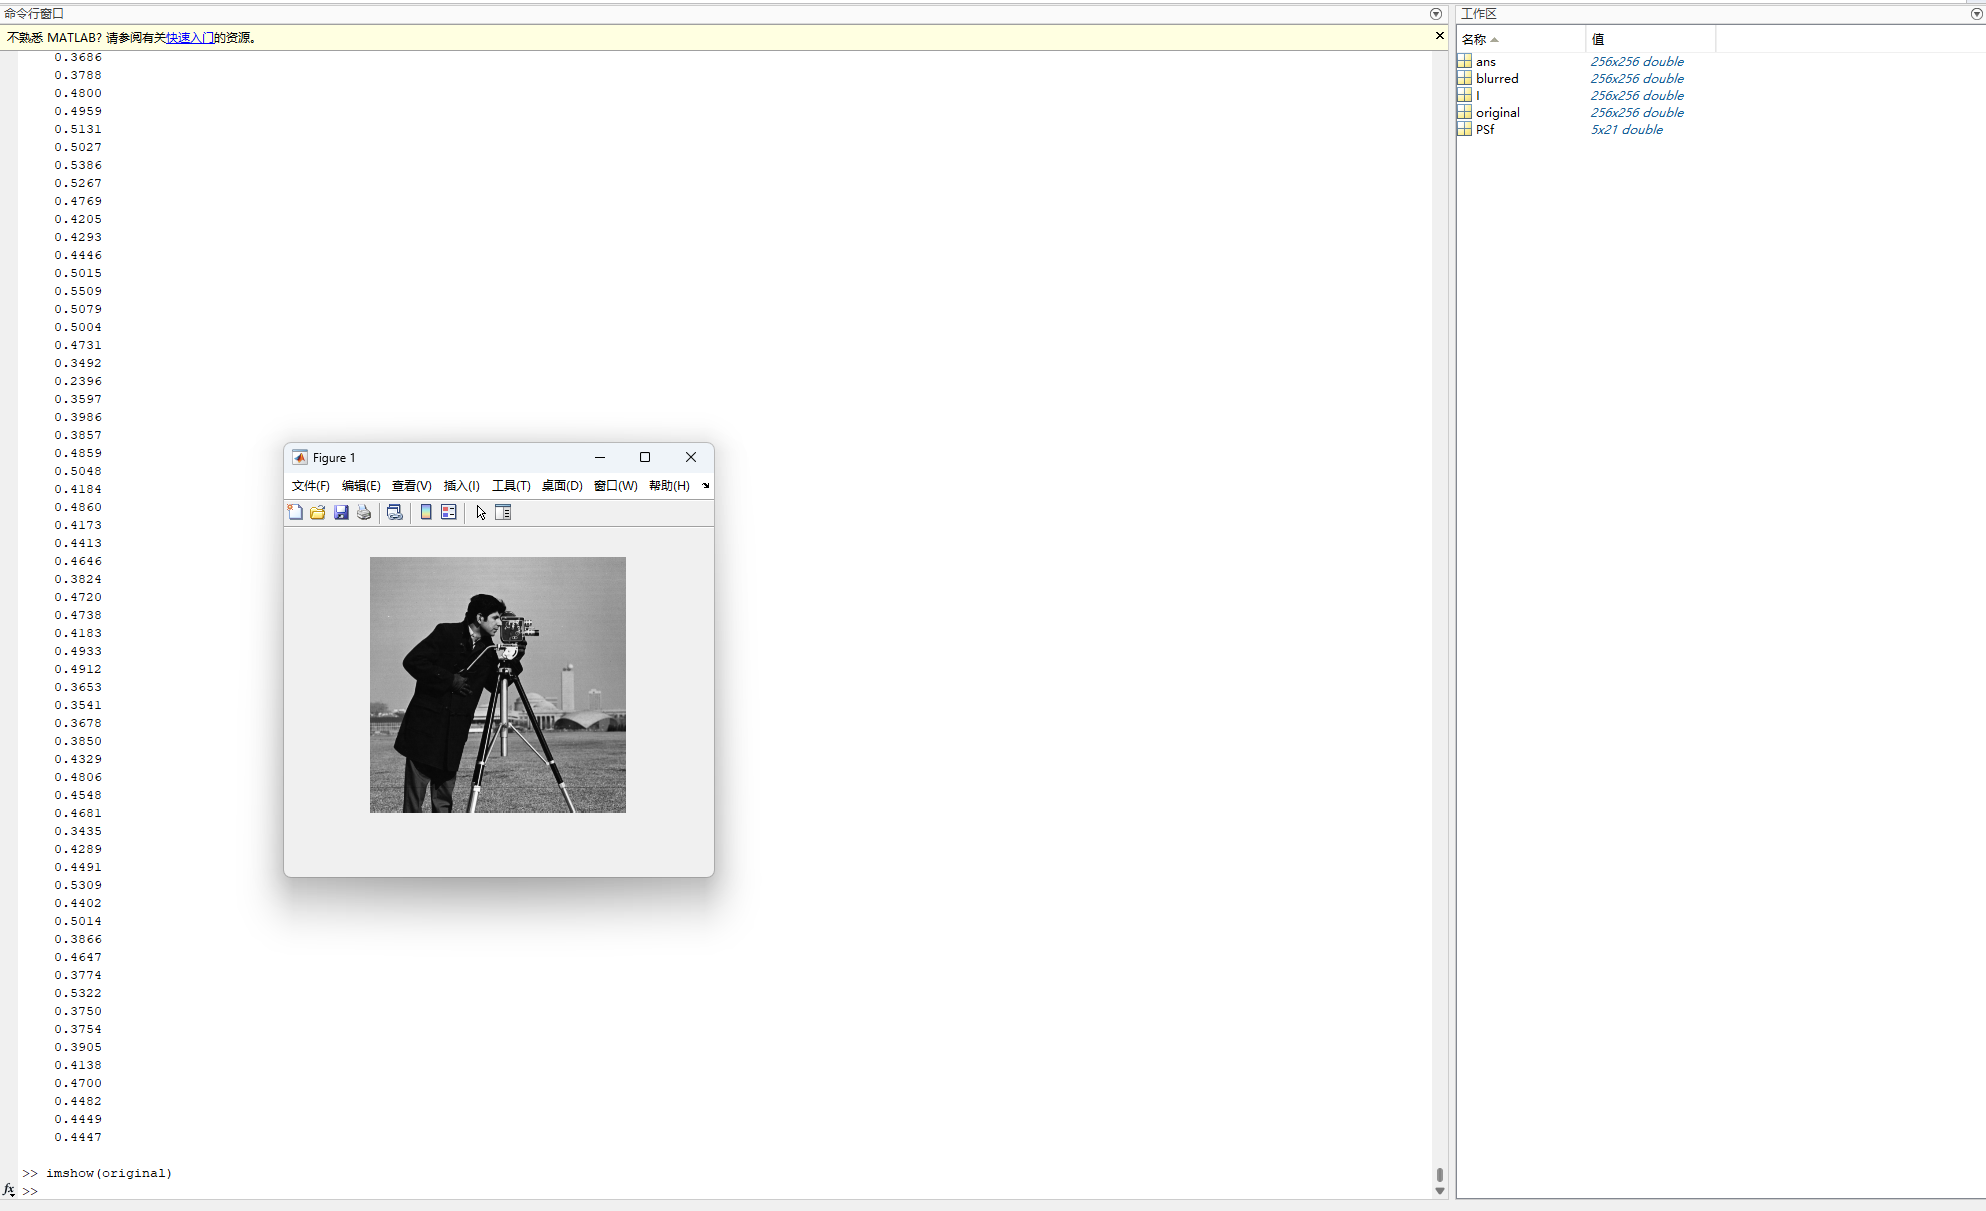
\includegraphics[width=\textwidth]{images/4-4-2.jpg}
    \caption{实验作业-2}\label{fig:4-2-1}
\end{figure*}
